\documentclass[a4paper, 12pt]{article}
\usepackage[spanish]{babel}
\usepackage[hmargin=2cm,vmargin=2.5cm]{geometry}
\usepackage{enumerate}
\usepackage{makecell}
\usepackage{graphicx}
\usepackage{hyperref}
\usepackage{amsmath}
\usepackage[backend=biber,style=apa, url=true, sortcites]{biblatex}
\usepackage[table]{xcolor}
\usepackage{minted}
\usepackage{graphicx}
\usepackage{fancyhdr}  % Agrega el paquete fancyhdr
\usepackage{subcaption}

\addbibresource{references.bib}
\hypersetup{
	colorlinks,
	citecolor=black,
	filecolor=black,
	linkcolor=black,
	urlcolor=black
}

\setlength{\arrayrulewidth}{0.4mm}

\newcommand{\HRule}{\rule{\linewidth}{0.5mm}}

\begin{document}
    \begin{titlepage}
        \begin{center}
            % logo
            
\includegraphics[width=0.5\textwidth]{figures/logoUAH.png}~\\[2cm]
            
            \textsc{\Large \\Sistemas de Control Inteligente}\\[2cm]
            
            \HRule \\[0.4cm]
            {\LARGE \bfseries Práctica 1. \\ Identificación y control neuronal  \\[0.4cm]}
            \HRule \\[3cm]
            
            \large\textbf{Jorge Revenga Martín de Vidales}\\
            \large\textbf{Ángel Salgado Aldao}\\
            \large\textbf{}\\ Grado en Ingeniería Informática \\ Universidad de Alcalá
            
            \vfill
            
            {\large \today}
        \end{center}
    \end{titlepage}

    % Configura los encabezados y pies de página
    \pagestyle{fancy}
    \fancyhf{} % Limpia todos los encabezados y pies de página actuales
    % Encabezado
    \fancyhead[RO,LE]{\textit{Sistemas de Control Inteligente}}
    \fancyhead[LO,RE]{\textit{Ejercicios de Introducción a Matlab}}  % Título del documento
    % Pie de página
    \fancyfoot[LO,RE]{\textit{Universidad de Alcalá}}
    \fancyfoot[RO,LE]{\thepage}  % Número de página en la esquina inferior derecha
    \newpage
    
    \thispagestyle{plain}
    \tableofcontents
    \newpage

    \part{}
    
    \section{Ejercicio 1. Perceptrón.}
    
	Se desea clasificar un conjunto de datos pertenecientes a cuatro clases diferentes.       Los datos y las clases a las que pertenecen con los que se muestra a continuación:
 
        \begin{figure}[htp!]
            \centering
            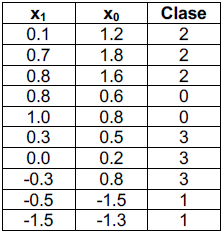
\includegraphics[width=0.25\textwidth]{Practica1/figures/parte1/Ej1/Ej1_fig0.png}
        \end{figure}

        Se desea diseñar un clasificador neuronal mediante un perceptrón simple que clasifique estos datos. Diseñe el clasificador, visualice los parámetros de la red y dibuje los datos junto con las superficies que los separan.
        
        \subsection{Código}
            \inputminted[fontsize=\scriptsize, linenos, breaklines=true, xleftmargin=0.75cm, frame=lines]{matlab}{code/parte1/Ej1.m}

        \subsection{Preguntas}
        
        \paragraph{¿Consigue la red separar los datos?}
            Sí, los clasifica en las 4 clases correctamente
    
        \paragraph{¿Cuántas neuronas tiene la capa de salida?, ¿por qué?}
        Tiene 4 neuronas, cada una genera una salida que representa la probabilidad de pertenencia a una clase particular, como tenemos 4 clases, tenemos 4 neuronas
    
        \paragraph{¿Qué ocurre si se incorpora al conjunto un nuevo dato: [0.0 -1.5] de la clase 3?}
        Las líneas que dividen los datos en las clases dejan de aplicarse a todos los datos, su pendiente ha cambiado pero el nuevo dato no está separado en el mismo espacio que el resto de datos de clase 3. Está con los datos de clase 1

        \newpage
	\subsection{Ejecución}
    	\begin{figure}[htp!]
    		\centering
    		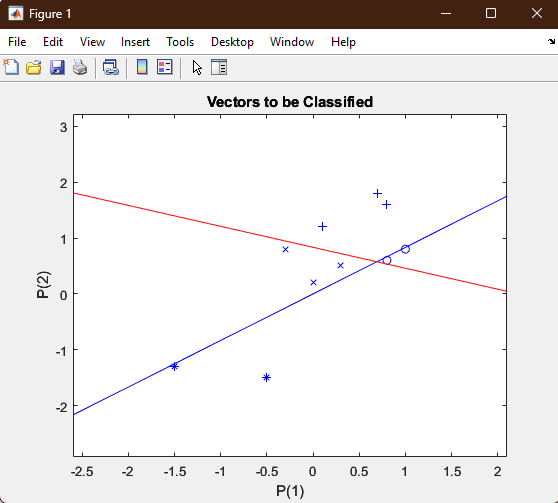
\includegraphics[width=0.69\textwidth]{figures/parte1/Ej1/Ej1_fig1.png}
    		\caption{Ejecución ejercicio 1.}
                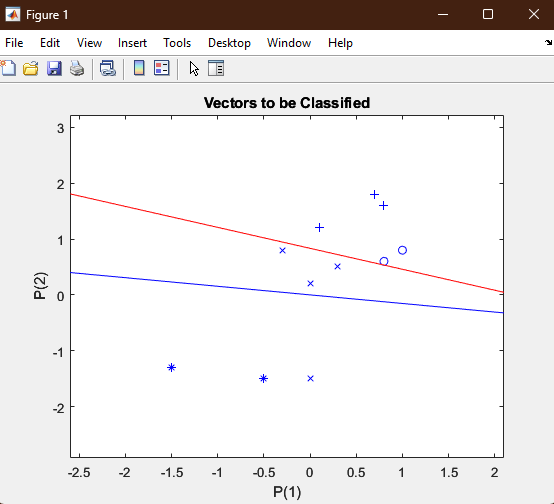
\includegraphics[width=0.69\textwidth]{figures/parte1/Ej1/Ej1_fig2.png}
        		\caption{Ejecución ejercicio 1 con el nuevo dato.}
    	\end{figure}
        \newpage

    
    \section{Ejercicio 2. Aproximación de funciones.}
    
        Una de las aplicaciones inmediatas de las redes neuronales es la aproximación de funciones. Para ello, Matlab dispone de una red optimizada, fitnet, con la que se trabajará en este ejercicio. El objetivo en este caso es aproximar la función \emph{f = sinc(t)} tal y como se muestra a continuación:

        \inputminted[fontsize=\scriptsize, linenos, breaklines=true, xleftmargin=0.75cm, frame=lines]{matlab}{code/parte1/Ej2.m}

        Estudie los efectos sobre la solución final de modificar el método de entrenamiento (consulte la ayuda de Matlab y pruebe 4 métodos diferentes) y el número de neuronas de la capa oculta.

        \subsection{Solución}
            Para poder visualizar el código en funcionamiento primero debemos definir la función \emph{sinc(t)}. Lo haremos en un archivo llamado sinc.m. En nuestro caso hemos definido la siguiente función \emph{sinc(t)}:

            \inputminted[fontsize=\scriptsize, linenos, breaklines=true, xleftmargin=0.75cm, frame=lines]{matlab}{code/parte1/sinc.m}

            \subsubsection{Ejecución}
                \begin{figure}[htp!]
                    \centering
    		      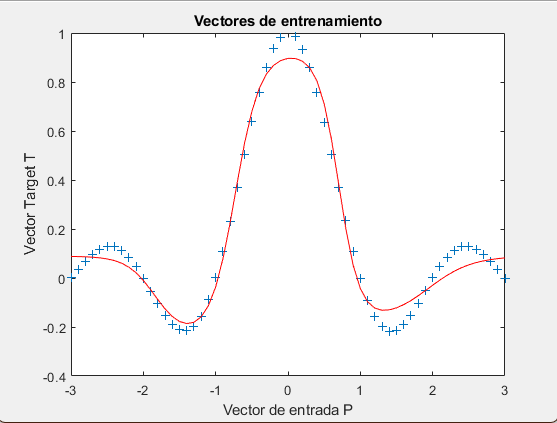
\includegraphics[width=0.7\textwidth]{figures/parte1/Ej2/Ej2_fig0_codigo_enunciado.png}
                \end{figure}
            
            Para modificar el método de entrenamiento basta con cambiar el segundo parámetro de la función \texttt{fitnet()} por otra función de entrenamiento. Vamos a estudiar las funciones \texttt{`traingd`} (descenso de gradiente), \texttt{`traingdm`} (descenso de gradiente con momento), \texttt{`trainlm`} (Levenberg-Marquardt), \texttt{`trainbr`} (Broyden-Fletcher-Goldfarb-Shanno).
            


 \end{document}